\chapter{Общие положения}

\section{Постановка задачи}

Пусть $T=\{t_1, t_2, \ldots, t_n\}$ --- множество временных меток наблюдений, а $d$ --- число метрик, собираемых системой. Для каждой метки $t_i$ формируется вектор значений:

\begin{equation}
	\mathbf{x}_i = [m^{(1)}_i, m^{(2)}_i, \ldots, m^{(d)}_i] \in \mathbb{R}^d,
\end{equation}

где компоненты соответствуют:
\begin{itemize}
	\item метрикам ML-конвейера: $timestamp\_sei$, $time\_delta\_$, $FPS\_$;
	\item метрикам бэкенда: $ml\_to\_backend\_kafka\_delay$, $db\_insert\_delay$;
	\item метрикам WS-клиента: $common\_event\_delay$, $heartbeat\_*$, $event\_counter$, $seq\_events\_health$.
\end{itemize}

Определим скользящее окно длины $L$ и шаг $s$. Каждое «окно»:

\begin{equation}
	X_k = [\mathbf{x}_{t_k - L + 1}, \ldots, \mathbf{x}_{t_k}] \in \mathbb{R}^{L \times d}.
\end{equation}

Целевая переменная --- значение end-to-end-задержки в следующий момент:

\begin{equation}
	y_k = common\_event\_delay(t_k + \Delta),\quad \Delta = 15\text{ с}.
\end{equation}

Обучающая выборка:

\begin{equation}
	\mathcal{N} = \{(X_k, y_k)\}_{k=1}^{N}.
\end{equation}

Существует неизвестная функция:

\begin{equation}
	f^*: \mathbb{R}^{L \times d} \to \mathbb{R},
\end{equation}

и задача состоит в построении алгоритма $A: \mathbb{R}^{L \times d} \to \mathbb{R}$ такого, что

\begin{equation}
	|A(X_k) - f^*(X_k)| \le \varepsilon,\quad \forall k.
\end{equation}

Требования к алгоритму $A$:

\begin{enumerate}
	\item Минимизировать среднеквадратическую ошибку MSE на валидационной выборке.
	\item Обеспечить $latency\_inference(A) < 1$ с в Docker-контейнере.
	\item Поддерживать периодическое дообучение (warm-start, frozen-слои, адаптеры/LoRNA).
	\item Гибкость частоты прогнозов: онлайн или с фиксацией интервала (например, 30 мин).
\end{enumerate}

Входные данные: многомерный временной ряд $X \in \mathbb{R}^{n \times d}$ (тип FLOAT64), формируемый из Prometheus по 30-секундным срезам ($\approx$90,644 точки за 16 дней).

Формализация задачи: построить алгоритм $A$, приближающий $f^*$, и удовлетворяющий указанным ограничениям по точности и latency.

\begin{landscape}
\vspace*{\fill}
\begin{figure}[H]
	\centering
	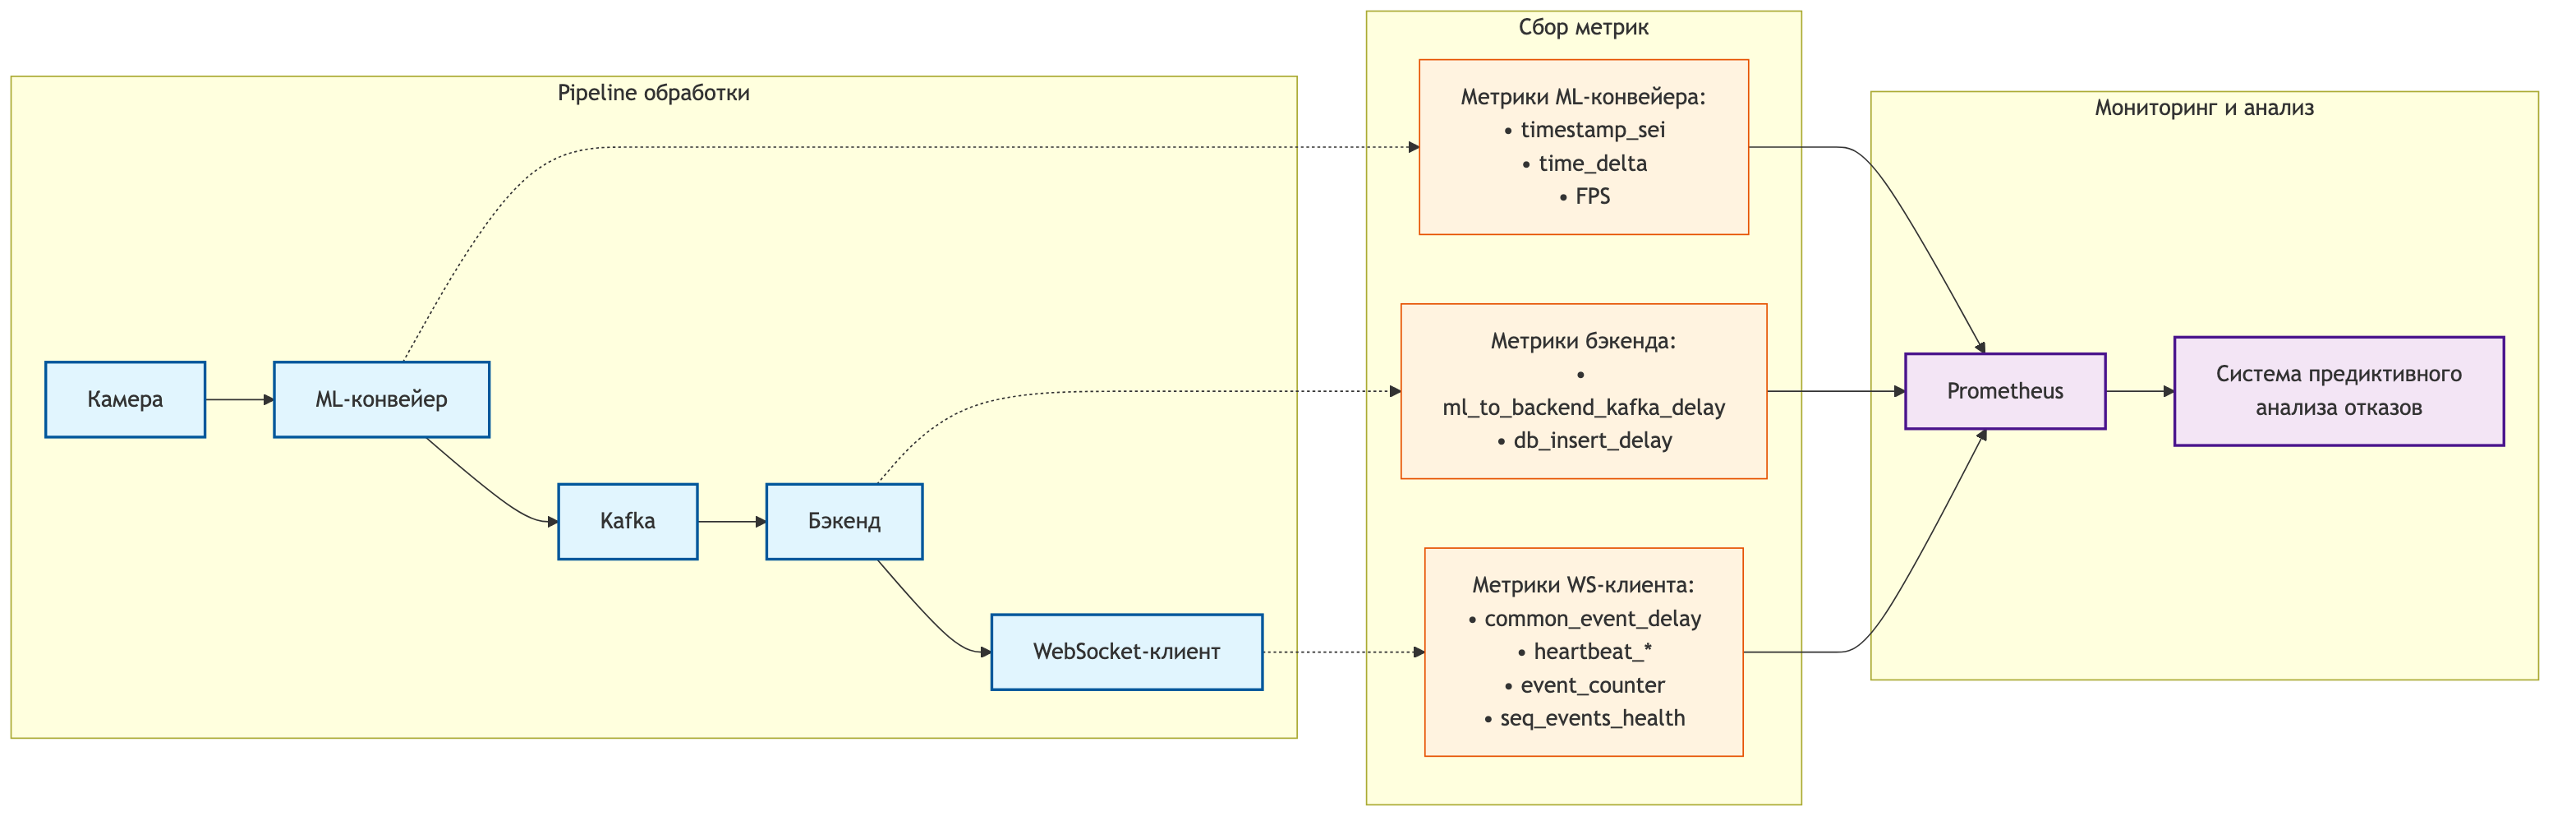
\includegraphics[width=\linewidth,height=\textheight,keepaspectratio]{figures/chapter1/video_pipeline_diagram.png}
	\caption*{Рисунок~1.1 --- Схема видеоконвейера и точки сбора метрик}
	\label{fig:video_pipeline}
\end{figure}
\vspace*{\fill}
\end{landscape}
